\section{Relationale Algebra}

Gegeben seien die Relationen R und S. Gilt die folgende Behauptung? Begründen Sie Ihre Antwort!

\texttt{PROJ(INTERSECT(R, S), E) = \beamertxt{\\ \hspace*{3em} =} INTERSECT(PROJ(R, E), PROJ(S, E))}

Umgangssprachlich: Dürfen Projektion und Schnittmenge vertauscht werden?

\begin{solution}
Die Behauptung gilt nicht.

Ein Gegenbeispiel: Gegeben seien die Relationen R und S:
\begin{center}
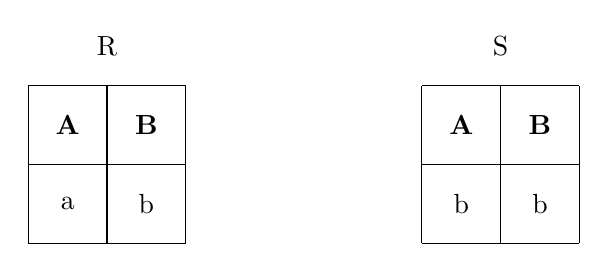
\begin{tikzpicture}
	\draw (0, 0) grid+(2, 2)
				(5, 0) grid+(2, 2);

	\node at(1, 2.5) {R};
	\node at(0.5, 0.5) {a};
	\node at(0.5, 1.5) {\textbf{A}};
	\node at(1.5, 0.5) {b};
	\node at(1.5, 1.5) {\textbf{B}};

	\node at(6, 2.5) {S};
	\node at(5.5, 0.5) {b};
	\node at(5.5, 1.5) {\textbf{A}};
	\node at(6.5, 0.5) {b};
	\node at(6.5, 1.5) {\textbf{B}};
\end{tikzpicture}
\end{center}

\texttt{PROJ(INTERSECT(R, S), B) = \{\}}, weil schon \texttt{INTERSECT(R, S) = \{\} }

Aber:
\texttt{INTERSECT(PROJ(R, B), PROJ(S, B)) = \{[b]\} }
\end{solution}

\begin{note}

\section*{Referenz: Vorlesungsfolien}

\paragraph{Hinweis:} Diese Umformungsregeln und Heuristiken werden in der Klausur \emph{nicht} angegeben.

\subsection*{Umformungsregeln}

\begin{enumerate}
	\item Ein n-facher Verbund kann durch eine Folge von binären Verbunden ersetzt werden und umgekehrt.
	\item Verbund ist kommutativ.
	\item Verbund ist assoziativ.
	\item Selektionen können zusammengefasst werden: \\
	\texttt{SEL(SEL(R,pred1),pred2) = SEL(R,(pred1 AND pred2))}
	\item Projektionen können zusammengefasst werden: \\
	\texttt{PROJ(PROJ(R,L1),L2) = PROJ(R,L2)}
	\item Projektion dürfen (in erweiterter Form) vorgezogen werden: \\
	\texttt{PROJ(SEL(R,pred(M)),L) = PROJ(SEL(PROJ(R,(L $\cup$ M)),pred(M)),L)}
	\item Selektion und Verbund dürfen vertauscht werden: \\
	\texttt{SEL(JOIN(R,S,pred1),pred2(R)) = JOIN(SEL(R,pred2),S,pred1)}
	\item Selektion darf mit Vereinigung und Differenz vertauscht werden: \\
	\texttt{SEL(UNION(R,S),pred) = UNION(SEL(R,pred),SEL(S,pred))}
	\item Selektion und Kreuzprodukt können zu Verbund zusammengefasst werden: \\
	\texttt{SEL(CROSS(R,S),pred) = JOIN(R,S,pred)}
\end{enumerate}


\subsection*{Heuristik zur Umformung}

\begin{itemize}
	\item \textbf{Komplexe Verbundoperationen zerlegen} in binäre Verbunde (Bilden von binären Verbunden)
	\item \textbf{Selektionen mit mehreren Prädikat-Termen separieren} in Selektionen mit jeweils einem Prädikat-Term
	\item \textbf{Selektionen so früh wie möglich ausführen}, d.\,h.\ Selektionen hinunterschieben zu den Blättern des Anfragegraphen (engl.\ selection push-down)
	\item \textbf{Selektionen und Kreuzprodukt zu Verbund zusammenfassen}, wenn das Selektionsprädikat Attribute aus den beiden Relationen verwendet
	\item \textbf{Einfache Selektionen wieder zusammenfassen}, d.\,h.\ aufeinanderfolgende Selektionen (derselben Relation) gruppieren
	\item \textbf{Projektionen so früh wie möglich ausführen}, d.\,h.\ Projektionen hinunterschieben zu den Blättern des Anfragegraphen, allerdings nicht vor die Selektion (engl.\ projection push-down); dabei aber die teure Duplikateliminierung vermeiden!
\end{itemize}
\pagebreak
\end{note}
